\textbf{TODO: find out laser parameters, LIA} 

The TSD setup (see Figure \ref{fig_TDS}) used for characterization of the fabricated H-Dipole antennas utilizes an ultrafast pulsed laser system. Bla bla bla...

The laser signal is coupled out using glass fibers. A beam splitter is utilized to split the initial laser pulse into two identical signals. One of the pulses is directly coupled to the receiving part (Rx) of the setup. The receiving part consists of an antenna that is being used to work as a recipient for THz radiation. For a PCA to work as a receiver, the device is illuminated by the femtosecond laser pulse. By illuminating the device, free electron-hole pairs are generated. The incoming THz radiation that is to be measured biases the device. The illumination and biasing of the device results in a photocurrent which is proportional to the THz field. As the measured photocurrent generally is very small (around $10^{-6} ... 10^{-9}$ \si{\ampere}), the signal is amplified by a trans-impedance amplifier (TIA).      

\begin{figure}[ht]
    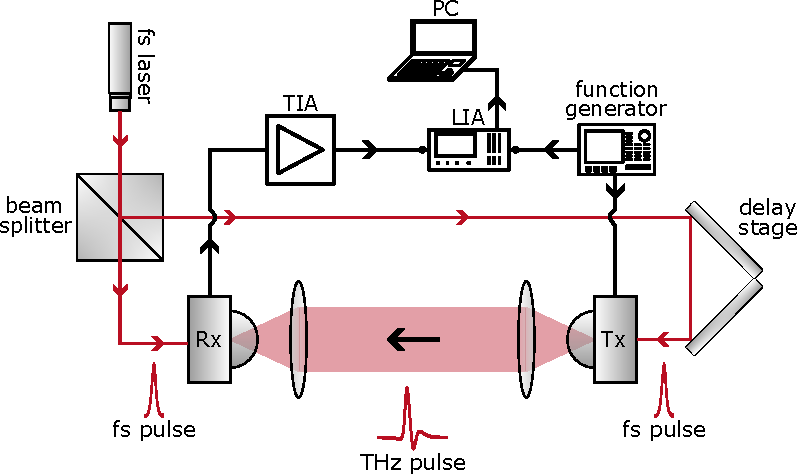
\includegraphics[width=0.9\linewidth]{figures/TDS_schematic.pdf}
    \centering
    \caption{Schematic diagram of the setup used for THz-TDS.}
    \label{fig_TDS}
\end{figure}

